\documentclass[11pt]{article}
\usepackage[a4paper,margin=1in]{geometry}
\usepackage{amsmath,amssymb,amsfonts}
\usepackage{graphicx}
\usepackage{booktabs}
\usepackage{float}
\usepackage[hidelinks]{hyperref}
\usepackage{xcolor}
\usepackage{enumitem}
\usepackage{array}
\graphicspath{{figures/}}

\title{\textbf{Roptimizer: A Multi-Stage High-Fidelity Framework for\\ Jump-Sensitive Portfolio Optimization}\\[4pt]
\large Tree-Structured Allocation, Scenario Bank Architecture, Hybrid DCC--Heston--Bates Dynamics,\\ and Empirical Jump Betas}
\author{Eljon Rrodhe\\[2pt]
\small Institutional Focus: Advanced Portfolio Engineering \& Quantitative Risk Management}
\date{\textbf{Version 5.0} \quad\textbullet\quad October 30, 2026}

\newcommand{\E}{\mathbb{E}}
\newcommand{\VIX}{\mathrm{VIX}}
\newcommand{\Var}{\mathrm{Var}}
\newcommand{\Cov}{\mathrm{Cov}}
\newcommand{\Corr}{\mathrm{Corr}}

\begin{document}
\maketitle

\begin{abstract}
\noindent Traditional portfolio construction rooted in Markowitz (1952) Mean--Variance Optimization (MVO)
fails to protect capital during systemic market stress because it assumes Gaussian asset returns, static
correlations, and deterministic volatility. This paper documents Version~5.0 of \textbf{Roptimizer}, an
open-source (Apache-2.0) institutional framework for jump-sensitive portfolio optimization. Roptimizer
replaces classical assumptions with high-fidelity physical and statistical dynamics: multivariate price paths
are generated by a \textbf{Hybrid DCC--Heston--Bates} simulation kernel featuring stochastic CIR variance,
discrete-time self-exciting (Hawkes) jump arrivals, Extreme Value Theory (EVT) Generalized Pareto shocks,
asymmetric variance co-jumps (SVJJ), forward-looking VIX volatility targeting, and a doubly adaptive
martingale jump compensator. Version~5.0 introduces five major architectural advances:
(1)~a \textbf{subportfolio tree} optimized bottom-up via post-order traversal using linear mixing matrices,
propagating limits and enforcing concentration penalties exclusively at the root;
(2)~a precomputed, GPU-resident \textbf{scenario bank} sized dynamically to hardware memory, featuring a
strictly held-out validation tenth that guarantees uncontaminated out-of-sample metrics;
(3)~a custom vectorized \textbf{Differential Evolution} engine with exact Euclidean projection onto boundary
and simplex constraints, paired generation-level draws, survivor re-scoring, and an early stopping rule;
(4)~an empirical \textbf{dated jump database} with per-asset crash and rally betas calibrated from S\&P~500
daily surprise days, alongside asymmetric variance co-jump multipliers; and
(5)~split-normal modeling of investor price targets and return views within a Black--Litterman framework.
We document rigorous computational benchmarks on laptop (NVIDIA RTX~3060) and cloud (NVIDIA A100) hardware,
report a regression check against the Version~4.1 reference answer, and compare the modeled tail metrics with
the production portfolio's own 2022--2026 history.
\end{abstract}

\begin{figure}[H]
\centering
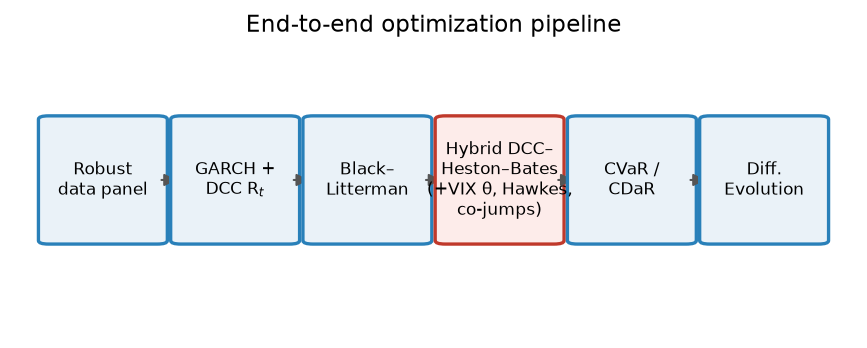
\includegraphics[width=\textwidth]{pipeline.png}
\caption{The end-to-end Roptimizer pipeline. Stages 1--3 estimate univariate volatility models, DCC correlations,
and Black--Litterman posterior drifts. Stage 4 simulates the joint scenario bank on GPU hardware. Stages 5--6
execute post-order subportfolio optimization targeting downside drawdown risk (UPI on CDaR) under exact
limit projections.}
\label{fig:pipeline}
\end{figure}

\section{Executive Summary}
Institutional asset managers face substantial tail risk when relying on classical portfolio models.
During liquidity contractions and market crashes, asset correlations converge rapidly toward unity, volatility
spikes discontinuously, and downside losses exhibit deep path dependency. Roptimizer Version~5.0 addresses these
vulnerabilities through an integrated, multi-stage architecture:
\begin{itemize}[nosep]
\item \textbf{Hierarchical Portfolio Tree:} Large asset universes are decomposed into modular subportfolios.
Each subportfolio is optimized independently, frozen, and represented as a single compound asset to its parent
through linear mixing matrices. Local and portfolio-wide limits are enforced at the appropriate hierarchy,
and Herfindahl concentration penalties are applied solely at the root on effective asset weights.
\item \textbf{GPU Scenario Bank:} Rather than re-simulating Monte Carlo paths at every candidate evaluation,
$2\times 10^6$ to $3\times 10^7$ joint asset paths are simulated once on the GPU and retained in memory.
A strictly held-out 10\% validation slice provides unbiased out-of-sample reporting for every row.
\item \textbf{Robust Differential Evolution:} Optimization utilizes a custom vectorized Differential Evolution
loop. Candidate vectors are projected onto linear simplex and inequality limits via bisection. Candidates and
survivors are scored across fresh bank draws, with survivor re-scoring preventing lucky Monte Carlo draws
from propagating inferior allocations.
\item \textbf{Empirical Jump Betas and Dated Database:} A persistent, dated jump database stores market-wide
jump intensities and per-asset crash and rally betas estimated on daily S\&P~500 surprise days, coupling
systematic tail shocks directly to asset volatilities and variance co-jumps.
\item \textbf{Split-Normal View Modeling:} Manager views expressed as target prices or annual returns with
asymmetric upside/downside uncertainties are mapped to exact split-normal moments and blended via Black--Litterman.
\item \textbf{Likelihood-Ratio GJR Selection and Short-History DCC:} Volatility models test for leverage
asymmetry via likelihood-ratio tests, assets lacking shock response are stabilized with constant-variance
refits, and DCC correlation dynamics are isolated to assets meeting an 80\% history threshold.
\item \textbf{Hybrid DCC--Heston--Bates Simulation:} Volatility follows mean-reverting stochastic CIR paths,
jumps arrive via discrete Hawkes cascades, and a state-dependent martingale compensator neutralizes drift distortion.
\end{itemize}

\section{Statistical Audit: The Normality Paradox}
Asset allocations based on variance implicitly assume that returns follow a multivariate normal distribution.
Operating in weekly log-return space for time-additivity, $r_t = \ln(P_t / P_{t-1})$, we evaluate normality
using the Jarque--Bera ($\mathrm{JB}$) statistic:
\begin{equation}
\mathrm{JB} = \frac{n}{6}\left( S^2 + \frac{(K-3)^2}{4}\right),
\end{equation}
where $n$ is sample length, $S$ is sample skewness, and $K$ is sample kurtosis. For essentially every risky
asset class (equities, digital assets, commodities), $\mathrm{JB}$ exceeds its critical value by orders of
magnitude. Real asset distributions exhibit pronounced negative skewness and excess kurtosis.
Linear covariance measures systematically understate the probability and depth of joint tail events,
necessitating non-Gaussian simulation and downside risk optimization.

\section{Robust Ingestion and Volatility Modeling}
\subsection{Data Ingestion and Calendar Synchronization}
Market data are cached by calendar day (\texttt{mso/data.py}) to eliminate runtime download latency and prevent
data drift across intra-day runs. All tickers are aligned to a shared weekly grid ending on Friday New York close.
Incomplete trading weeks in progress are automatically dropped, ensuring that estimation parameters remain
invariant to the timing of execution within the week.

\subsection{Univariate Volatility: GARCH, GJR, and Constant-Variance Refits}
Financial assets exhibit heterogeneous histories. Truncating all assets to the shortest common history
discards valuable data on established tickers. Roptimizer fits univariate volatility models on each asset's
full history.

\paragraph{Likelihood-Ratio Leverage Gate.}
For each asset with at least 104 weekly observations (\texttt{gjr\_min\_obs}), Roptimizer fits both a standard
symmetric $\mathrm{GARCH}(1,1)$ and an asymmetric $\mathrm{GJR-GARCH}(1,1,1)$ model:
\begin{align}
r_t &= \mu + \epsilon_t, \quad \epsilon_t = \sigma_t z_t, \quad z_t \sim \mathcal{N}(0, 1), \\
\sigma_{t,\mathrm{GJR}}^2 &= \omega + \big(\alpha + \gamma\,\mathbf{1}_{\{\epsilon_{t-1} < 0\}}\big)\epsilon_{t-1}^2 + \beta\,\sigma_{t-1}^2.
\end{align}
An asymmetric down-shock increases next-period variance by $(\alpha + \gamma)\epsilon_{t-1}^2$, whereas an
up-shock increases variance by $\alpha\,\epsilon_{t-1}^2$. The framework evaluates the likelihood-ratio statistic:
\begin{equation}
\mathrm{LR} = 2\left(\ln L_{\mathrm{GJR}} - \ln L_{\mathrm{GARCH}}\right) \sim \chi^2(1).
\end{equation}
If $p = \Pr(\chi^2(1) \ge \mathrm{LR}) < 0.05$ (\texttt{gjr\_alpha}) and the fit converges, GJR is retained;
otherwise, the asset defaults to plain GARCH. The implied Heston leverage correlation $\rho_i$ is computed
from the standardized residuals $z_t$ and the asymmetric shock:
\begin{equation}
\rho_i = \Corr\big(z_t,\, (\alpha + \gamma\,\mathbf{1}_{\{z_t < 0\}}) z_t^2\big),
\end{equation}
clipped to $[-0.95, 0.95]$. If plain GARCH is retained, $\rho_i = 0$, eliminating spurious correlation from
symmetric shocks.

\paragraph{Constant-Variance Refit.}
When an asset exhibits near-zero responsiveness to return shocks ($\alpha + \gamma/2 < 10^{-3}$, defined as
\texttt{NO\_SHOCK\_RESPONSE} in \texttt{mso/fits.py}), the maximum-likelihood $\mathrm{GARCH}$ variance
merely decays exponentially from its initialization, failing to identify $\omega$ and $\beta$. On real 5-year
weekly panels, a strongly trending name can trigger this condition; for NVDA the GARCH
current variance came out 40\% under its realized level. Roptimizer identifies this condition at fit
time and refits the asset as a \texttt{ConstantVariance} process anchored to its historical realized variance:
\begin{equation}
\sigma_{i, t}^2 = \sigma_{i, \mathrm{realized}}^2.
\end{equation}
During Heston CIR calibration, mean reversion $\kappa_i$ and the relative vol-of-vol ratio
$\xi_i / \sqrt{\theta_i}$ are pooled from identified assets in the portfolio (using the median values),
while $\rho_i$ is set to 0. Every pooled fit is explicitly labeled in diagnostic logs.

\subsection{Multivariate Dependence: DCC with Short Histories}
Multivariate correlations are modeled using Dynamic Conditional Correlation (Engle, 2002).
The conditional covariance matrix decomposes as $H_t = D_t R_t D_t$, with $D_t = \mathrm{diag}(\sigma_{1,t},\dots,\sigma_{N,t})$
and dynamic correlation matrix:
\begin{equation}
R_t = \mathrm{diag}(Q_t)^{-1/2}\,Q_t\,\mathrm{diag}(Q_t)^{-1/2}, \qquad
Q_t = (1-a-b)\bar{Q} + a(\eta_{t-1}\eta_{t-1}^{\top}) + b\,Q_{t-1},
\end{equation}
where $\eta_t = D_t^{-1}\epsilon_t$ are standardized residuals and $\bar{Q}$ is the unconditional target.
The parameters $a, b \ge 0$, $a+b < 0.999$, are estimated via Gaussian quasi-maximum likelihood (QML):
\begin{equation}
\min_{a, b}\ \frac{1}{2}\sum_{t=1}^T \left(\ln|R_t| + \eta_t^{\top} R_t^{-1} \eta_t\right).
\end{equation}
If $\hat{a} < 10^{-4}$, the data support no dynamic correlation, and $a, b$ are set to zero.

\paragraph{The 80\% Short-History Rule.}
When assets have disparate history lengths, intersecting all assets to a common window severely truncates the
sample (e.g., an asset with 126 weeks would force all 260-week series down to 126 weeks).
In \texttt{mso/fits.forecast\_dcc}, Roptimizer applies the 80\% short-history rule:
\begin{itemize}[nosep]
\item Assets with observation counts $n_i \ge 0.80 \times \max_j(n_j)$ carry the dynamic correlation filter.
The dynamic recursion $Q_t^{(dyn)}$ is calibrated on their shared overlap.
\item Assets with shorter histories ($n_i < 0.80 \times \max_j(n_j)$) are excluded from the dynamic filter.
Their rows and columns in the forecasted $Q_t$ are held fixed at their unconditional pairwise correlations
$\bar{Q}_{ij}$ (estimated on their individual complete pair overlaps).
\item If the resulting composite correlation matrix $R_t$ violates positive semi-definiteness, it is repaired
per step via eigenvalue clipping:
\begin{equation}
R_t \leftarrow \sum_{k=1}^N \max(\lambda_k, 10^{-8}) v_k v_k^{\top}, \quad
R_t \leftarrow \mathrm{diag}(R_t)^{-1/2} R_t \mathrm{diag}(R_t)^{-1/2}.
\end{equation}
\end{itemize}

\section{Views, Split-Normal Moments, and Black--Litterman}
\subsection{View Forms and Horizon Compounding}
Investor views in Roptimizer (\texttt{mso/views.py}) can be entered either as an annual expected return $m$
or as a target price $P_{\mathrm{target}}$ over horizon $h$ (default 12 months). A target price is annualized
via compounding against the current asset price $P_0$:
\begin{equation}
m = \left(\frac{P_{\mathrm{target}}}{P_0}\right)^{12/h} - 1.
\end{equation}

\subsection{Asymmetric Uncertainty and Split-Normal Moments}
Portfolio managers frequently possess asymmetric confidence (e.g., expecting a stock to reach \$200 from \$180,
with downside risk of \$10 but upside potential of \$20). Roptimizer requires explicit minus ($-s_-$) and
plus ($+s_+$) uncertainties in return points or dollar ranges. There are no defaults: a view without both
uncertainties blocks the run.
Dollar ranges are converted to annual return bounds:
\begin{equation}
s_- = \left|\left(\frac{P_{\mathrm{target}} - \Delta \$_-}{P_0}\right)^{12/h} - 1 - m\right|, \qquad
s_+ = \left|\left(\frac{P_{\mathrm{target}} + \Delta \$_+}{P_0}\right)^{12/h} - 1 - m\right|.
\end{equation}
Treating $m$ as the mode of a two-piece (split-normal) distribution with left standard deviation $s_-$
and right standard deviation $s_+$, the exact mean $\mu_{\mathrm{view}}$ and variance $\sigma_{\mathrm{view}}^2$
are derived from split-normal moment equations:
\begin{align}
\mu_{\mathrm{view}} &= m + \sqrt{\frac{2}{\pi}}\,(s_+ - s_-), \\
\sigma_{\mathrm{view}}^2 &= \left(1 - \frac{2}{\pi}\right)(s_+ - s_-)^2 + s_+\,s_-.
\end{align}
For example, a price of \$180 with target \$200 (mode $+11.1\%$) and $-\$10 / +\$20$ bounds yields an effective
input of $+15.5\% \pm 8.5\%$.

\subsection{Black--Litterman Posterior Blending}
Views are blended with CAPM equilibrium returns $\Pi$ via Theil's mixed estimator (\texttt{mso/bl.py}):
\begin{equation}
\E[R] = M_{\mathrm{post}} \left[(\tau\Sigma)^{-1}\Pi + P^{\top}\Omega^{-1}Q\right], \qquad
M_{\mathrm{post}} = \left[(\tau\Sigma)^{-1} + P^{\top}\Omega^{-1}P\right]^{-1}.
\end{equation}
The prior uncertainty parameter is fixed at $\tau = 0.01$, reflecting institutional commitment to the
efficient-market anchor ($\sqrt{\tau} = 10\%$ of asset volatility). The view covariance $\Omega$ is
$\mathrm{diag}(\sigma_{\mathrm{view}, i}^2)$ in annual units, matching $\Sigma$ and $\Pi$ exactly.
The posterior covariance matrix $M_{\mathrm{post}}$ captures parameter uncertainty and is retained for
subportfolio view blending and sensitivity bands.

\section{Empirical Jump Betas and the Dated Jump Database}
\subsection{The Dated Jump Database}
Systematic and idiosyncratic tail shocks are maintained in a versioned, dated jump database (\texttt{jumpdb/},
e.g., \texttt{jumpdb/2026-10-29/}). Re-calibrated offline over an editable 406-ticker pool (\texttt{pool.json}),
the database stores calibrated Hawkes intensities, Pareto parameters, and jump betas.

\subsection{Surprise Days and Empirical Jump Betas}
Market surprise days are identified from daily S\&P~500 (\nolinkurl{^GSPC}) log returns.
A $\mathrm{GARCH}(1,1)$ filter with a constant mean on daily data (\nolinkurl{mso/betas.py}) isolates standardized residuals:
\begin{equation}
D_{\mathrm{crash}} = \{t : z_t^{\mathrm{SP}} < -3\}, \qquad
D_{\mathrm{rally}} = \{t : z_t^{\mathrm{SP}} > +3\}.
\end{equation}
For each asset $i$, crash and rally betas are computed from its overlapping daily log returns:
\begin{equation}
\beta_{\mathrm{crash}, i} = \frac{\frac{1}{|D_{\mathrm{crash}}|}\sum_{t \in D_{\mathrm{crash}}} r_{i, t}}{\frac{1}{|D_{\mathrm{crash}}|}\sum_{t \in D_{\mathrm{crash}}} r_{\mathrm{SP}, t}}, \qquad
\beta_{\mathrm{rally}, i} = \frac{\frac{1}{|D_{\mathrm{rally}}|}\sum_{t \in D_{\mathrm{rally}}} r_{i, t}}{\frac{1}{|D_{\mathrm{rally}}|}\sum_{t \in D_{\mathrm{rally}}} r_{\mathrm{SP}, t}}.
\end{equation}
When an asset history contains fewer than 10 surprise days (\texttt{MIN\_DAYS}), a fallback hierarchy applies:
\begin{enumerate}[nosep]
\item \textbf{Stocks (EQUITY):} Betas are obtained from a non-parametric LOWESS regression of jump beta on standard OLS
beta, calibrated across all modelled pool stocks with $\ge 2400$ daily returns ($\approx 10$ years) and $\ge 3$
surprise days (LOWESS smoothing spans: 0.6 for crash, 0.5 for rally).
\item \textbf{Non-stocks (ETFs, futures, funds):} Fallback to the standard full-sample OLS beta $\beta_{\mathrm{normal}, i}$.
\item \textbf{Manual overrides:} Stored in \texttt{library/beta\_overrides.json}, surviving database recalibrations.
\end{enumerate}

\subsection{Systematic Jumps and Variance Co-Jumps in the Simulator}
In the simulation engine (\texttt{mso/sim.py}), a systematic jump $J$ drawn from the Generalized Pareto
distribution (in z-score units) affects asset $i$ according to:
\begin{equation}
\Delta \ln S_{i, t}^{\mathrm{sys}} = \beta_i(J) \cdot J \cdot \sigma_{m, t}, \qquad
\beta_i(J) = \begin{cases} \beta_{\mathrm{crash}, i}, & J < 0 \\ \beta_{\mathrm{rally}, i}, & J > 0 \end{cases}
\end{equation}
where $\sigma_{m, t}$ is the S\&P~500 weekly conditional volatility forecast over the horizon from an $\mathrm{AR}\text{--}\mathrm{GARCH}$
fit on weekly bars. On a systematic crash ($J < 0$), asset $i$'s instantaneous variance receives an asymmetric
co-jump proportional to its \emph{current} variance:
\begin{equation}
v_{i, t} \leftarrow v_{i, t} + m_i\,v_{i, t}, \qquad m_i \sim \mathrm{Exp}(\mathrm{mean} = \mathrm{cojump}_i),
\end{equation}
where $\mathrm{cojump}_i$ is the empirical mean proportional rise in asset $i$'s weekly conditional variance following
historical S\&P~500 crash weeks ($z_t^{\mathrm{SP}} < -3$ on weekly bars, requiring $\ge 3$ weeks; otherwise
defaulting to the market pooled multiplier). Idiosyncratic crashes apply the pooled multiplier to current variance.

\section{Hybrid DCC--Heston--Bates Dynamics}\label{sec:heston}
Each asset's price and variance follow a continuous-time stochastic process with self-exciting Hawkes jumps:
\begin{align}
\frac{dS_i}{S_i} &= \mu_i\,dt + \sqrt{v_i}\,dW^{S}_i + \Big(e^{\Delta \ln S_i^{\mathrm{jump}}}-1\Big)\,dN_i, \\
dv_i &= \kappa_i(\theta_{i,t} - v_i)\,dt + \xi_i\sqrt{v_i}\,dW^{v}_i + m_i\,v_i\,dN^{\mathrm{crash}}_i, \\
\mathrm{corr}(dW^{S}_i, dW^{v}_i) &= \rho_i, \qquad \mathrm{corr}(dW^{S}_i, dW^{S}_j) = R_{t,ij}.
\end{align}
Parameters $\kappa_i, \theta_i, \xi_i$ are calibrated from the historical conditional-variance series $v_t = \sigma_t^2$
via the discrete Euler regression $\Delta v_t = a + b\,v_{t-1} + \epsilon_t$, yielding $\kappa = -b/\Delta t$,
$\theta = a/(\kappa\Delta t)$, and $\xi^2 = \E[\epsilon_t^2] / (v_{t-1}\Delta t)$, enforcing the floor $\xi \ge 10^{-4}$.
Initial variance $v_{0, i}$ is initialized to the GARCH one-step-ahead forecast $\sigma_{T+1}^2$.

\begin{figure}[H]
\centering
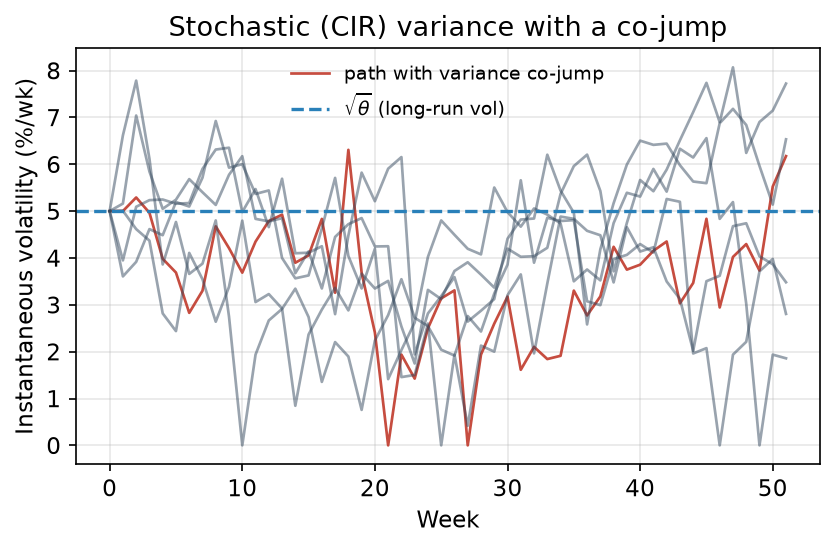
\includegraphics[width=0.72\textwidth]{cir_paths.png}
\caption{Stochastic CIR variance paths mean-reverting toward $\sqrt{\theta}$. The highlighted red path receives
an empirical crash-triggered variance co-jump (SVJJ), elevating post-crash volatility.}
\end{figure}

\subsection{VIX-Driven Long-Run Target Tilt}\label{sec:vixtheta}
The long-run variance target $\theta_{i, t}$ is tilted by the current level of the VIX relative to its historical mean:
\begin{equation}
r_i = \mathrm{clip}\!\left(\Big(\tfrac{\VIX_{\text{now}}}{\overline{\VIX}}\Big)^{\gamma_i},\,0.5,\,3.0\right),
\qquad r_{i,t} = 1 + (r_i-1)\,e^{-\rho t},
\qquad \theta'_{i,t} = \theta_{i,t}\,r_{i,t}.
\end{equation}
The elasticity $\gamma_i$ is the regression slope of $\ln v_{i,t}$ on $\ln \VIX_t$. The tilt decays toward neutral
over the 12-week horizon ($\rho = 0.3$), capturing market mean-reversion.

\begin{figure}[H]
\centering
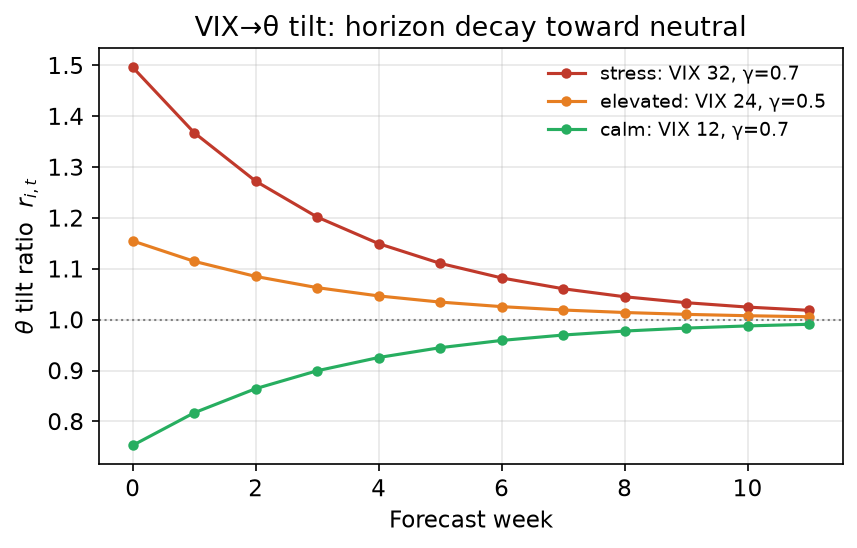
\includegraphics[width=0.72\textwidth]{vix_decay.png}
\caption{The VIX$\to\theta$ tilt ratio $r_{i, t}$ decays exponentially back to neutral across the forecast horizon.}
\end{figure}

\subsection{Modelling Market Extremes: Asymmetric Pareto Jumps}\label{sec:jumps}
Jumps are calibrated via the Generalized Pareto Distribution (GPD) on normalized exceedances beyond threshold $u = 3.0$:
\begin{equation}
G_{\xi,\beta}(x) = 1 - \left(1 + \frac{\xi(x-u)}{\beta}\right)^{-1/\xi}.
\end{equation}
Systemic dates ($|z_t^{\mathrm{SP}}| > 3$, crashes and rallies) are filtered out before calibrating idiosyncratic tails, preventing
double-counting. Tail shape parameters are capped at $\xi \le 0.3$ for numerical stability.

\begin{figure}[H]
\centering
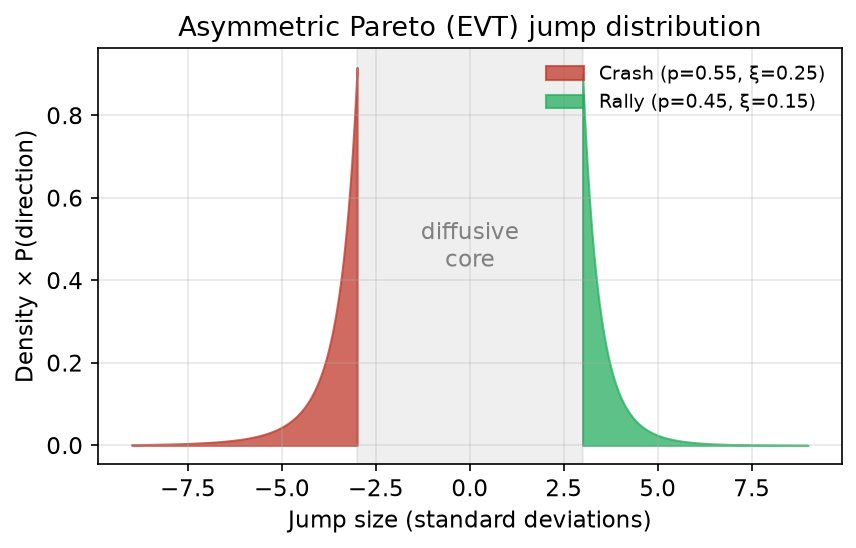
\includegraphics[width=0.66\textwidth]{jump_density.png}
\caption{Asymmetric truncated Pareto jump distributions: heavier crash distribution versus lighter rally tail,
surrounding a diffusive Gaussian core.}
\end{figure}

\subsection{Hawkes Arrival Intensities}
Jump intensities follow a discrete-time Hawkes process:
\begin{equation}
\lambda_t = \lambda_\infty + (\lambda_{t-1}-\lambda_\infty)\,e^{-\alpha} + \beta\,\mathbf{1}\{\text{jump at } t-1\},
\end{equation}
producing crisis cascades. Stationarity requires the branching ratio $\beta / (1 - e^{-\alpha}) < 1$; calibration caps it at $0.95$.

\section{The Jump-Drift (Martingale) Compensator}\label{sec:comp}
Adding asymmetric jumps shifts the simulated drift away from the Black--Litterman posterior.
The discrete log-price step incorporates a state-dependent martingale compensator:
\begin{equation}
\Delta\ln S_{i, t} = \ln(1+\mu_i) - \tfrac{1}{2}v_{i,t}\Delta t - \mathrm{comp}_{i, t}\Delta t + \sqrt{v_{i,t}\Delta t}\,Z_i^S + \Delta\ln S_{i, t}^{\mathrm{jump}}.
\end{equation}
For idiosyncratic jumps, the compensator evaluates $g(s) = \E[e^{J s} - 1 \mid \text{jump}]$ tabulated over
volatility $s = \sqrt{v}$ on a uniform grid ($N=513$, Common Random Numbers):
\begin{equation}
\mathrm{comp}_{\mathrm{idio}, i, t} = \lambda_{\mathrm{idio}, i, t} \cdot g_{\mathrm{idio}}(\sqrt{v_{i, t}}).
\end{equation}
For systematic jumps, the compensator incorporates asset betas and market volatility (\nolinkurl{mso/sim._beta_compensator}):
\begin{equation}
g_{\mathrm{sys}, i}(t) = \E\Big[e^{\mathrm{clip}(\beta_i(J) J \sigma_{m, t},\, -5,\, 5)} - 1 \;\Big|\; \text{systematic jump}\Big],
\end{equation}
evaluated deterministically per step $t$ and asset $i$. Total compensation is given by:
\begin{equation}
\mathrm{comp}_{i, t} = \lambda_{\mathrm{sys}, t} g_{\mathrm{sys}, i}(t) + \lambda_{\mathrm{idio}, i, t} g_{\mathrm{idio}}(\sqrt{v_{i, t}}) \mathbf{1}_{\{i \notin \mathrm{exempt}\}}.
\end{equation}

\begin{figure}[H]
\centering
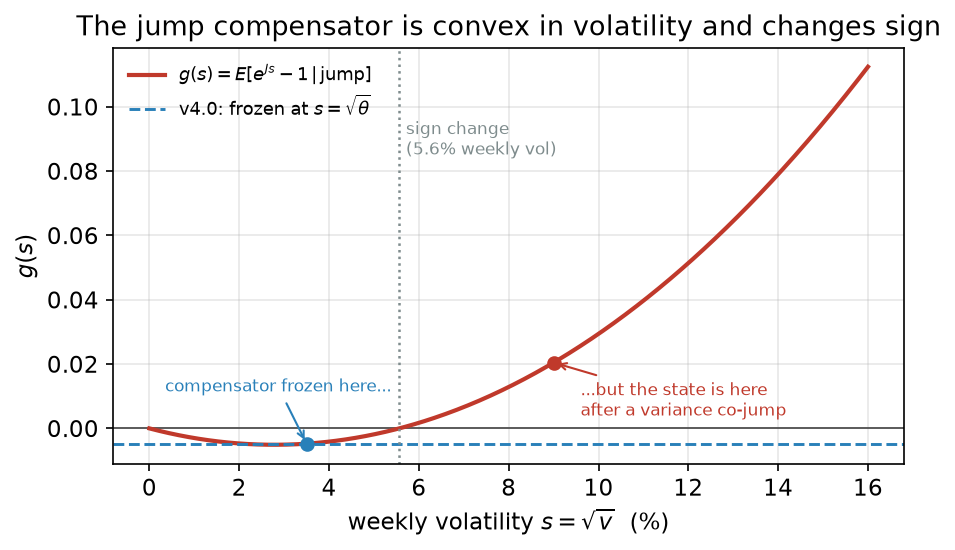
\includegraphics[width=0.74\textwidth]{compensator.png}
\caption{The jump compensator curve $g(s) = \E[e^{Js}-1 \mid \text{jump}]$ as a function of volatility $s=\sqrt{v}$.
Frozen evaluation at $\sqrt{\theta}$ fails under post-crash variance spikes where $g(s)$ changes sign.}
\label{fig:comp}
\end{figure}

\section{Tail Risk Metrics: CVaR and CDaR}
Downside risk is quantified by coherent measures. Conditional Value at Risk ($\mathrm{CVaR}_\alpha$) measures
mean terminal losses in the worst $\alpha = 5\%$ tail:
\begin{equation}
\mathrm{CVaR}_\alpha(X) = \E[X \mid X \le \mathrm{VaR}_\alpha(X)].
\end{equation}
For path-dependent drawdowns with running peak $\mathrm{Peak}(t) = \max_{0 \le \tau \le t} P(\tau)$ and
drawdown $D(t) = (P(t) - \mathrm{Peak}(t)) / \mathrm{Peak}(t) \le 0$, Conditional Drawdown at Risk
($\mathrm{CDaR}_\alpha$) is the average of the worst $\alpha$ maximum drawdowns across all scenarios:
\begin{equation}
\mathrm{CDaR}_\alpha = \frac{1}{\lfloor \alpha M \rfloor} \sum_{m=1}^{\lfloor \alpha M \rfloor} \mathrm{MDD}_{(m)}.
\end{equation}

\section{The Scenario Bank Architecture}
In Version~4.1, differential evolution executed independent Monte Carlo simulations per candidate, incurring
massive GPU simulation overhead. Version~5.0 decouples simulation from search through a precomputed
\textbf{Scenario Bank} (\texttt{mso/bank.py}).

\subsection{Memory Layout and GPU Planning}
The scenario bank is a contiguous 3D \texttt{float32} tensor of cumulative return paths $R_{i, t}(s)$, stored
in path-major layout $(\text{paths}, \text{assets}, \text{steps})$ on the GPU. Sizing is governed by \texttt{bank.plan()}:
\begin{equation}
\text{Memory} = M \times N \times T \times 4\text{ bytes}.
\end{equation}
For $N=16$ assets, $T=12$ weeks, and $M=30\times 10^6$ paths on a 40~GB NVIDIA A100 GPU, the bank occupies
$21.46\text{ GiB}$ ($1.34\text{ GiB}$ per asset). \texttt{bank.plan()} allocates memory across two phases:
\begin{enumerate}[nosep]
\item \textbf{Build Phase:} Allocates the persistent bank tensor plus one simulation chunk (312 bytes per path-asset peak memory).
\item \textbf{Search Phase:} Allocates the bank, a gathered draw buffer ($2\times \text{draw} \times N \times T \times 4$ bytes),
and candidate scoring scratch buffers ($2\times \text{draw} \times 64 \times 4$ bytes).
\end{enumerate}
On laptop hardware (6~GB RTX~3060), \texttt{bank.plan()} provisions 2M paths; on Colab A100, 30M paths.

\subsection{The Held-Out Validation Slice}
The scenario bank is partitioned into a 90\% searchable training subset and a strictly held-out 10\% validation
subset (e.g., 200k paths on laptop, 3M paths on A100). Optimization searches draw randomly from the 90\% slice.
Every metric, fan quantile, and histogram reported in final results is calculated on the held-out slice.
No reported number is ever measured on paths the search evaluated.

\section{Optimization Engine: Differential Evolution on the Bank}
Version~5.0 replaces the external SciPy optimizer with an in-house vectorized Differential Evolution engine
(\texttt{mso/search.py}) tailored for GPU scenario evaluation.

\subsection{Vectorized Best-1-Bin Search}
The population size is $P = \mathrm{pop\_per\_dim} \times n$ (default $30 \times n$). Initial vectors are
generated via Latin hypercube sampling and projected onto the feasible constraint set. At each generation $g$:
\begin{itemize}[nosep]
\item A mutation vector is formed around the current best vector: $v_i = x_{\mathrm{best}} + F (x_{r_1} - x_{r_2})$,
with a mutation factor $F \sim \mathcal{U}(0.5, 1.0)$ drawn once per generation (dither).
\item Binomial crossover occurs with probability $\mathrm{CR} = 0.7$, forcing at least one parameter exchange.
\item The trial vector is projected onto linear limits.
\end{itemize}

\subsection{Exact Simplex and Bound Projection}
Unlike heuristic clipping, \texttt{search.project} computes the exact Euclidean projection of an arbitrary
vector $v$ onto the bounded simplex $\{w \in \mathbb{R}^n : lo_i \le w_i \le hi_i, \sum w_i = 1\}$:
\begin{equation}
w_i^*(\mu) = \mathrm{clip}(v_i - \mu,\, lo_i,\, hi_i), \qquad \sum_{i=1}^n w_i^*(\mu) = 1.
\end{equation}
The shift parameter $\mu$ is solved via bisection over 60 iterations, guaranteeing absolute precision.

\subsection{Generation-Level Draws and Survivor Re-scoring}
In each generation, a fresh random subset of paths ($M_{\mathrm{draw}} = 10^6$ on laptop, $3\times 10^6$ on A100)
is drawn from the searchable bank. Both the current population and candidate mutants are evaluated on this
\emph{identical draw} in a single batched kernel. A mutant replaces its parent if and only if it achieves a superior
score on that paired draw.

\paragraph{Why Re-scoring Exists.}
In a stochastic simulation, an inferior weight vector can occasionally receive an unusually benign scenario draw
(a ``lucky draw''). If evaluated only once, such a candidate would permanently pollute the population.
To prevent this, Roptimizer maintains a running average score for every surviving candidate:
\begin{equation}
\bar{f}_{c+1} = \frac{\bar{f}_c \cdot c + f_{\mathrm{new}}}{c + 1}, \qquad c \leftarrow c + 1.
\end{equation}
The search incumbent is selected as the candidate with the lowest running mean among those evaluated at least
twice ($c \ge 2$).

\subsection{Early Stopping Rule and Objective Function}
The search terminates when the incumbent's running average objective improves by less than $\mathrm{tol} = 0.0002$
over a 5-generation window ($g > 5$ and $\bar{f}_{g-5} - \bar{f}_g < 0.0002$), subject to a maximum cap of 80 generations.
In the benchmark studies the rule stopped searches at generations 6--8. Scored on the held-out paths, the
answer at the stop matched the generation-80 answer within $0.00001$ for most searches; where it differed
(small subportfolios) the earlier answer was the better one, by up to $0.0046$.

\paragraph{Objective Formulation.}
The search minimizes the penalized negative Ulcer Performance Index on CDaR:
\begin{equation}
\min_w\ -\left(\frac{\E[R_p] - R_f}{|\mathrm{CDaR}_\alpha|} - \lambda_{\mathrm{HHI}}\sum_{i=1}^N A_i^2\right)
+ \lambda_{\mathrm{floor}} \max(0,\, \mathrm{CVaR}_{\mathrm{floor}} - \mathrm{CVaR}_\alpha),
\end{equation}
with concentration weight $\lambda_{\mathrm{HHI}} = 0.20$ (applied at root on effective weights $A$, 0 inside
subportfolios), soft floor weight $\lambda_{\mathrm{floor}} = 5.0$, and ruin threshold $\mathrm{CVaR}_{\mathrm{floor}} = -40\%$.

\section{Hierarchical Allocation: The Portfolio as a Tree}
Version~5.0 formalizes portfolio structure as an arbitrary-depth directed tree (\texttt{mso/tree.py}).

\subsection{Post-Order Bottom-Up Traversal}
The tree is solved in post-order (leaves first, bottom-up). When subportfolio $k$ is optimized, its internal
weights $w_k^*$ are frozen. To its parent node, subportfolio $k$ behaves exactly as a single synthetic asset.
Its path in any scenario is linear in its components through mixing matrix $M_k$:
\begin{equation}
R_{\mathrm{sub}, t}(s) = \sum_{i=1}^{n_k} w_{k, i}^* R_{i, t}(s) = \big(M_k w_k^*\big)^{\top} R_t(s).
\end{equation}
No additional bank columns, re-simulations, or parameter refits are required.

\subsection{Mixing Matrices and Effective Weights}
For any node at depth $d$, the mapping from its local allocation vector $w$ to underlying physical assets
is given by mixing matrix $M \in \mathbb{R}^{N \times K}$, where column $j$ is the frozen asset weight vector
of child $j$. The portfolio-wide effective weight vector $A \in \mathbb{R}^N$ is the product along the tree path:
\begin{equation}
A = M_{\mathrm{root}} w_{\mathrm{root}}^* = \prod_{\mathrm{path}} w_{\mathrm{node}}^*.
\end{equation}

\subsection{Limit Propagation and Squeezes}
Each child node supports independent local limits $lo_k \le w_k \le hi_k$. Whole-portfolio limits
$[\underline{W}_n, \overline{W}_n]$ specified on an arbitrary nested node $n$ are projected up to the
top-level child $c$ holding node $n$:
\begin{equation}
w_c \le \frac{\overline{W}_n}{S_{n|c}}, \qquad w_c \ge \frac{\underline{W}_n}{S_{n|c}},
\end{equation}
where $S_{n|c}$ is the internal share of node $n$ within top child $c$ (the product of frozen shares down the branch).
These bounds squeeze the local search range $[lo_c, hi_c]$ of the top-level child, reporting infeasibilities
prior to search execution.

\subsection{Subportfolio View Blending and Sensitivity Bands}
When an investor expresses a view $(q_r, \sigma_r)$ on a subportfolio group, its implied annual return
$imp_k = \mu^{\top} (M w)_k$ and covariance $\Sigma_{jk} = (M w)_j^{\top} M_{\mathrm{post}} (M w)_k$ are blended
using Black--Litterman mixed estimation at the parent level:
\begin{equation}
\mu_{\mathrm{blended}} = imp + \Sigma P^{\top}\big(P \Sigma P^{\top} + \Omega\big)^{-1}(q - P\,imp),
\end{equation}
shifting the parent's expected return without perturbing the frozen internal mix $w_k^*$.
An optional sensitivity band (off by default) repeats the search $K$ times drawing asset returns from $\mathcal{N}(\mu, M_{\mathrm{post}})$,
reporting 10th--90th percentile weight intervals.

\section{Comprehensive Out-of-Sample Performance Ratios}
Roptimizer reports an extensive battery of risk-adjusted ratios on the held-out validation paths
(\texttt{mso/report.py}), summarized in Table~\ref{tab:ratios}.

\begin{table}[H]
\centering
\caption{Comprehensive performance and tail ratios computed on held-out validation scenarios ($T = 12$ weeks,
$ex = \E[R_p] - R_f$, $d_t = R_{p, t} - R_f$).}
\label{tab:ratios}
\small
\setlength{\tabcolsep}{3pt}
\begin{tabular}{llp{6.4cm}}
\toprule
Ratio / Metric & Mathematical Definition & Description \\
\midrule
Sharpe (Horizon / Ann.) & $\frac{ex}{\sigma(R_p)} \ \Big[\times \sqrt{52/T}\Big]$ & Return per unit of total terminal standard deviation \\
Sortino (Horizon / Ann.) & $\frac{ex}{\sqrt{\E[\min(d_t, 0)^2]}} \ \Big[\times \sqrt{52/T}\Big]$ & Return penalized by semi-deviation below risk-free rate \\
UPI & $\frac{ex}{|\mathrm{CDaR}_\alpha|}$ & Ulcer Performance Index: return per unit of tail drawdown \\
STARR & $\frac{ex}{-\mathrm{CVaR}_\alpha}$ & Stable Tail Adjusted Return Ratio relative to expected shortfall \\
Calmar & $\frac{ex}{-\E[\mathrm{MDD}]}$ & Excess return normalized by expected maximum drawdown \\
Martin & $\frac{ex}{\mathrm{Ulcer}}, \ \mathrm{Ulcer} = \E\big[\sqrt{\frac{1}{T}\sum_{t=1}^T D_t^2}\big]$ & Return per unit of path-dependent Ulcer quadratic drawdown \\
Omega & $\frac{\E[\max(d_t, 0)]}{\E[\max(-d_t, 0)]}$ & Ratio of upside probability mass to downside loss mass \\
Rachev & $\frac{\E[R_p \mid R_p \ge q_{1-\alpha}]}{-\mathrm{CVaR}_\alpha}$ & Ratio of extreme right-tail gains to extreme left-tail losses \\
Skewness & $\E\big[\big(\frac{R_p - \bar{R}_p}{\sigma}\big)^3\big]$ & Asymmetry of terminal return distribution \\
Excess Kurtosis & $\E\big[\big(\frac{R_p - \bar{R}_p}{\sigma}\big)^4\big] - 3$ & Leptokurtosis and fat-tail thickness relative to Gaussian \\
\bottomrule
\end{tabular}
\end{table}

\section{Computational Engineering and Hardware Telemetry}
Roptimizer executes across dual hardware backends: CuPy on CUDA GPU devices and NumPy on host CPUs.
Table~\ref{tab:benchmarks} summarizes measured hardware execution times recorded during release testing
(October 29, 2026, \nolinkurl{README.md}).

\begin{table}[H]
\centering
\caption{Measured hardware performance across local laptop and cloud GPU environments.}
\label{tab:benchmarks}
\small
\setlength{\tabcolsep}{4pt}
\begin{tabular}{p{4.2cm}p{5.1cm}p{5.5cm}}
\toprule
Metric / Task & Laptop NVIDIA RTX 3060 (6 GB) & Colab NVIDIA A100 (40 GB SXM4) \\
\midrule
Scenario Bank Generation & 2M paths in 5.6--8.2 s & 30M paths in 9.5--21.9 s \\
DE Generation (16-asset flat) & 6.0 s per gen (1M-path draws) & 6.0 s per gen (3M-path draws) \\
Reference Tree (8 searches) & 64 s search wall time & 67 s search wall time \\
Full Run, 16 Assets & 71 s (reference tree) & 163--181 s (incl.\ 58 s VM start-up) \\
Cloud Compute Billing & Local free compute & 5.30 Compute Units / hour \\
\bottomrule
\end{tabular}
\end{table}

\section{Empirical Validation and Regression Tests}\label{sec:val}
\subsection{Regression Check Against Version~4.1 Reference}
To guarantee that architectural modularization did not impair numerical fidelity, Roptimizer requires a
flat-portfolio regression test against the Version~4.1 reference answer
(\nolinkurl{benchmarks/reference/inputs.json}, 16 assets, 12 weeks, $R_f = 1.13\%$). Re-scored at 10M paths,
the Version~4.1 benchmark established a reference score of $-0.08833$ (standard deviation $0.00004$).
The reference inputs carry no per-asset jump betas, so this check covers the new scenario bank and search, not
the Version~5.0 jump features; $R_f$ is the 12-week rate.
Version~5.0 achieves:
\begin{itemize}[nosep]
\item \textbf{Laptop RTX~3060:} $-0.08987$ (superior / lower objective value).
\item \textbf{Colab A100:} $-0.08993$ (also lower).
\end{itemize}

\subsection{Historical Tail Check}
To verify that modeled tails are realistic rather than artificially optimistic, the Version~5.0 production
allocation was backtested against historical overlapping 12-week windows across 242 weeks (2022-03-07 to 2026-10-19)
using weekly closes from the day cache (\nolinkurl{benchmarks/results/slice7/tail-check.md}). The window lies
inside the 5-year estimation window and the weights are held fixed, so this is a consistency check of the
simulated tails against the same portfolio's history, not an out-of-sample test. Table~\ref{tab:tailcheck}
reports the results.

\begin{table}[H]
\centering
\caption{12-week tail comparison: Historical realization vs Version~5.0 simulated bank (A100,
3M held-out paths).}
\label{tab:tailcheck}
\small
\setlength{\tabcolsep}{5pt}
\begin{tabular}{lrr}
\toprule
Metric (12-week, 5\% tail) & History (242 weeks) & Simulated (3M Paths) \\
\midrule
Mean Return & $+2.72\%$ & $+2.73\%$ \\
Volatility & $5.61\%$ & $5.58\%$ \\
CVaR (5\%) & $-7.31\%$ & $-7.94\%$ \\
CDaR (5\%) & $-9.25\%$ & $-9.92\%$ \\
Worst Realized 12-Week Loss & $-11.42\%$ (from 2022-03-21) & Modeled in severe tail \\
\midrule
\multicolumn{3}{p{11.5cm}}{\emph{Common 127-week window (all assets live):} History CVaR $-5.66\%$, CDaR $-8.22\%$ vs Simulated $-7.94\%$, $-9.92\%$} \\
\bottomrule
\end{tabular}
\end{table}

\noindent The simulated tails are more conservative than the realized ones: by about 0.6 points of CVaR for the
portfolio over the full window, 2.3 points over the 127 weeks where every asset has history, and much more for a
single volatile asset (BTC=F simulated CVaR $-40.8\%$ against a historical $-26.7\%$), verifying that Roptimizer's jump clustering and variance
co-jumps enforce genuine downside defensiveness without distorting expected return.

\subsection{Foundational Component Validation (Version~4.1 Baseline)}
The physical validity of the underlying simulation kernels was established in Version~4.1 on a 7-asset panel
(261 weekly bars, 400k paths, 12-week horizon) under common random seeds. Table~\ref{tab:ladder} and
Figure~\ref{fig:ladder} reproduce the ladder demonstrating monotonic deepening of tail risk under invariant drift.

\begin{table}[H]
\centering
\caption{Engine ladder: component marginal tail-risk contribution under Version~4.1 state-dependent compensator
(400k paths, common seeds, from \texttt{paper/main.tex} v4.1 study).}
\label{tab:ladder}
\small
\setlength{\tabcolsep}{4.5pt}
\begin{tabular}{lrrrrrr}
\toprule
Engine & mean ret & std & CVaR(5\%) & CDaR(5\%) & ex.\ kurt & $\overline{r}\,|\,\mathrm{DD}_{10}$ \\
\midrule
1. Legacy GBM            & 0.0236 & 0.168 & $-0.287$ & $-0.251$ & 0.70 & $-0.217$ \\
2. Heston (no jumps)     & 0.0224 & 0.125 & $-0.210$ & $-0.181$ & 0.01 & $-0.162$ \\
3. \ + Bates jumps       & 0.0222 & 0.166 & $-0.286$ & $-0.250$ & 0.73 & $-0.218$ \\
4. \ + Hawkes clustering & 0.0221 & 0.177 & $-0.312$ & $-0.270$ & 1.94 & $-0.223$ \\
5. \ + Variance co-jumps & 0.0221 & 0.184 & $-0.338$ & $-0.285$ & 3.62 & $-0.234$ \\
\bottomrule
\end{tabular}
\end{table}

\begin{figure}[H]
\centering
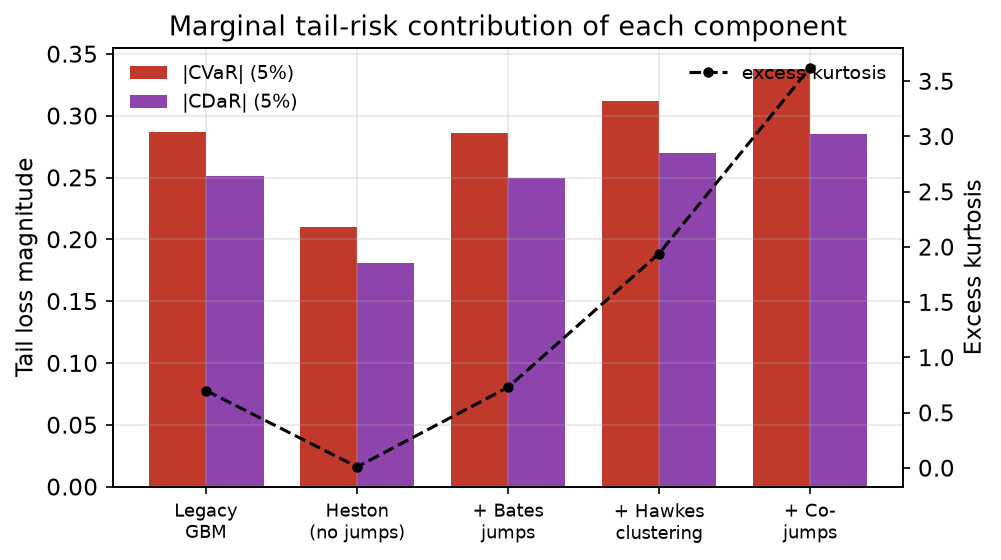
\includegraphics[width=0.74\textwidth]{ladder.png}
\caption{Tail risk and kurtosis increase monotonically as Bates jumps, Hawkes clustering, and variance co-jumps
are enabled, while mean returns remain stable.}
\label{fig:ladder}
\end{figure}

\noindent Table~\ref{tab:comp_ab} confirms the necessity of state-dependent compensator tracking against the
legacy frozen-$\sqrt{\theta}$ formulation:

\begin{table}[H]
\centering
\caption{Full engine under frozen vs state-dependent compensators (identical data and seeds, v4.1 study).}
\label{tab:comp_ab}
\small
\begin{tabular}{lrrr}
\toprule
Metric & v4.0 frozen $\sqrt{\theta}$ & v4.1 state-dependent & Change \\
\midrule
Mean return                         & 0.0232   & 0.0221   & $-0.0011$ \\
CVaR(5\%)                           & $-0.3342$ & $-0.3381$ & $-1.2\%$ \\
CDaR(5\%)                           & $-0.2829$ & $-0.2853$ & $-0.9\%$ \\
Excess kurtosis                     & 3.46     & 3.62     & $+4.5\%$ \\
$\overline{r}\,|\,\mathrm{DD}_{10}$ & $-0.2299$ & $-0.2340$ & $-1.8\%$ \\
\bottomrule
\end{tabular}
\end{table}

\noindent Table~\ref{tab:rallysens} demonstrates that allocation weights are robust to rally tail variations,
with between-group spread (0.53 pp) remaining well below optimizer noise (1.25 pp).

\begin{table}[H]
\centering
\caption{Mean optimal allocation weights across rally-tail shapes (v4.1 study, 3 seeds each).}
\label{tab:rallysens}
\small
\begin{tabular}{lrrrr}
\toprule
Ticker & $\xi_{\text{rally}}=0.08$ & $0.12$ (base) & $0.16$ & $\Delta$ \\
\midrule
PLTR   &  3.61\% &  2.65\% &  2.78\% & $-0.82$ pp \\
NVDA   & 13.64\% & 12.91\% & 12.32\% & $-1.32$ pp \\
META   & 10.96\% & 12.13\% & 12.42\% & $+1.46$ pp \\
JPM    & 24.37\% & 23.39\% & 23.20\% & $-1.16$ pp \\
GOOGL  & 18.09\% & 18.37\% & 18.60\% & $+0.50$ pp \\
FERG   & 18.63\% & 19.53\% & 19.11\% & $+0.49$ pp \\
BTC=F  & 10.71\% & 11.00\% & 11.57\% & $+0.86$ pp \\
\midrule
\multicolumn{5}{l}{Within-group spread (same shape, different seed): \textbf{1.25 pp} average per name} \\
\multicolumn{5}{l}{Between-group spread (attributable to shape): \textbf{0.53 pp} average per name} \\
\bottomrule
\end{tabular}
\end{table}

\section{Algorithmic Walkthrough}
To execute Version~5.0 end to end:
\begin{enumerate}[nosep]
\item \textbf{Data Ingestion:} Load cached daily-aligned weekly prices; drop incomplete trading bars; compute weekly log returns.
\item \textbf{Univariate Modeling:} Fit $\mathrm{GARCH}(1,1)$; execute likelihood-ratio test for $\mathrm{GJR}(1,1,1)$; refit assets with $\alpha + \gamma/2 < 10^{-3}$ as constant variance.
\item \textbf{Multivariate Correlation:} Estimate pairwise correlations; filter dynamic DCC recursion to assets with $\ge 80\%$ of longest history; embed short-history assets in $\bar{Q}$; repair positive semi-definiteness via eigenvalue clipping.
\item \textbf{Heston CIR Calibration:} Calibrate $\kappa_i, \theta_i, \xi_i, \rho_i, v_{0, i}$; pool constant-variance parameters from identified assets; tilt long-run targets $\theta_{i, t}$ by forward-looking VIX elasticity with horizon decay.
\item \textbf{Tail Jumps and Betas:} Load dated jump database; extract S\&P~500 surprise days; compute direct or LOWESS/normal fallback crash and rally betas; calibrate empirical variance co-jump multipliers.
\item \textbf{Bayesian Drift Blending:} Transform price/return views into split-normal moments; compute Black--Litterman posterior returns and covariance ($\tau = 0.01$).
\item \textbf{Scenario Bank Allocation:} Provision GPU memory via \texttt{bank.plan()}; simulate joint cumulative return tensor; partition into 90\% search and 10\% held-out validation slices.
\item \textbf{Hierarchical Tree Search:} Perform post-order bottom-up search; project candidate vectors onto limits; evaluate generations on fresh bank draws; re-score surviving candidates; propagate mixing matrices and squeeze parent limits; penalize HHI concentration at root.
\item \textbf{Held-Out Reporting:} Compute comprehensive out-of-sample ratios (Sharpe, Sortino, UPI, STARR, Calmar, Martin, Omega, Rachev) and generate fan charts on the held-out slice.
\end{enumerate}

\section{Conclusion}
Roptimizer Version~5.0 bridges institutional portfolio theory and modern high-performance quantitative engineering.
By pairing a Hybrid DCC--Heston--Bates simulation core with empirical crash/rally jump betas, hierarchical tree
structures, GPU-accelerated scenario banks, and projection-constrained Differential Evolution, the framework
delivers rigorous, provably defensive allocations under severe market turbulence. The complete codebase,
benchmarks, and documentation are published under the open-source Apache-2.0 license for institutional research
and quantitative deployment.

\end{document}
